% PREAMBLE Version 0.1

% DO NOT COMPILE THIS FILE ALONE

% Document classes
% ----------------
\documentclass[a4paper, 11pt, oneside]{article}
% \documentclass[a4paper,landscape]{article}

% Project structure
% -----------------
\usepackage{subfiles}

% Spacing, margins, etc.
% ----------------------
\usepackage{geometry}
\usepackage{float}
\usepackage{fullpage}
\usepackage{indentfirst}
\usepackage[francais]{babel}
% \usepackage[english]{babel}

% Encoding, characters, fonts, etc.
% ---------------------------------
\usepackage[T1]{fontenc}
\usepackage[utf8]{inputenc}
% \usepackage{upgreek}
\usepackage{eurosym}
\usepackage{amsfonts}
\usepackage{amssymb}
\usepackage{textcomp}

% Figures
% -------
\usepackage{graphicx}
% \usepackage{subfigure}

% Colors
% ------
% \usepackage{color}
\usepackage[table]{xcolor}

% URLs and refs
% -------------
% \usepackage{url}
% \usepackage{hyperref}
% \usepackage[bottom]{footmisc}
% \usepackage[all]{hypcap}

% Environments
% ------------
\usepackage{amsmath}
\usepackage{amsthm}
\usepackage{array}
\usepackage{tabularx}
\usepackage{enumerate}
\usepackage{enumitem}
\usepackage{listings}
\usepackage{framed}
\usepackage[framed]{matlab-prettifier}
\usepackage{booktabs}
\usepackage{algorithm}
\usepackage{algorithmic}

% =================================================================================
%                                   New commands
% =================================================================================



\renewcommand{\thesubsection}{\alph{subsection})}
\renewcommand{\thesubsubsection}{\roman{subsubsection})}
\usepackage{clrscode3e}

\begin{document}

\subfile{titlepage.tex}

\section{Répartition des cases} %1
%Ton boulot drewdrew <3
\subsection{} %a
\subsection{} %b
\subsection{} %c
\subsection{} %d
\subsection{} %e

\setcounter{section}{0}

\section{Calcul de la couture d'énergie minimale} %1
%Mon boulot
\subsection{} %a
Une approche exhaustive consisterait à calculer le coût de tous les chemins possibles puis de chercher celui avec le coût minimal.
Pour atteindre le pixel (i, j), i étant la dernière ligne:

Si la hauteur = 1, 1 chemin possible.

Si la hauteur = 2, 3 chemins possibles.\footnote{Si le pixel est au bord de l'image alors il n'y a que 2 chemins possibles, mais on ne va pas considérer ce cas ici pour plus de simplicité}

Si la hauteur = 3, $3*3=9$ chemins possibles.

Si la hauteur = n, $3*3*...=3^{n-1}$ chemins possibles.

L'approche exhaustive est donc bien de complexité exponentielle.
\subsection{} %b
Cas de base, $i = 0$, $j \in [0, largeur - 1]$ ;

 $C(i, j)$ = $E(i, j)$
\bigbreak
$\forall i > 0, j \in [0, largeur - 1]$ tels que $C(i - 1, j -1)$, $C(i - 1, j)$ et $C(i - 1, j + 1)$ sont définis :

$C(i, j) = E(i, j) + min(C(i - 1, j -1), C(i - 1, j), C(i - 1, j + 1))$\footnote{Si j - 1 ou j + 1 dépassent les limites de l'image, on n'en tient pas compte dans le calcul du minimum.}
\subsection{} %c
\begin{figure}[H]
	\centering
	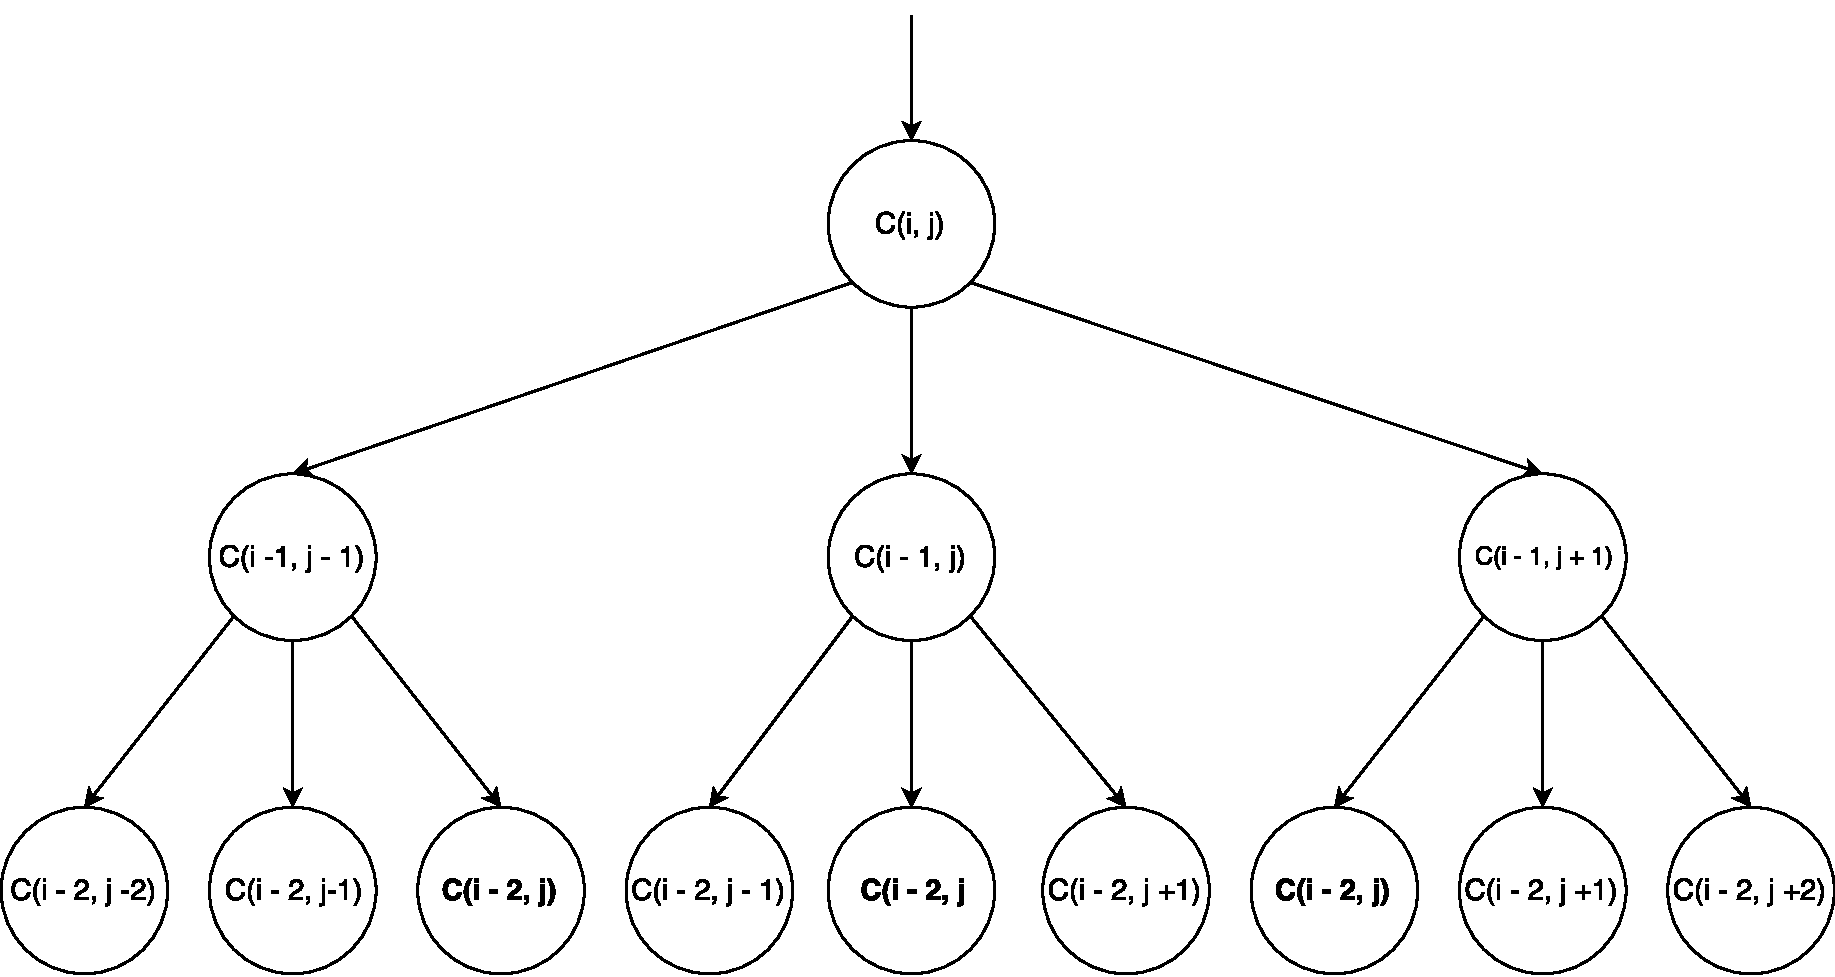
\includegraphics[width=1\linewidth]{cost.pdf}
	\caption{Graphe des appels récursifs}
	\label{cost}
\end{figure}

On peut voir dans la figure \ref{cost} que l'on effectue plusieurs fois le même appel (en gras). Afin de ne pas faire inutilement des calculs, on tâchera de retenir les valeurs déjà calculées.

\subsection{} %d
\begin{codebox}
\Procname{$\proc{Cost}(energy)$}
\li \For $j = 1$ \To $width$
\Do
\li 	$cost[1][j] = energy[1][j]$
\End
\li \For $i = 2$ \To $heigth$
\Do 
\li 	\For $j = 1$ \To $width$
 		\Do
\li 		\If $j - 1> 1$
			\Do 
\li 			$left = cost[i - 1][j - 1]$
\End
\li 		$mid = cost[i - 1][j]$
\li 		\If $j + 1< width$
			\Do 
\li 			$right = cost[i - 1][j + 1]$
\End
\li \Comment Si left ou right n'est pas défini, on en tient pas compte
\li 		$cost[i][j] = energy[i][j] + min(left, mid, right)$
	\End
\End
\li \Return $cost$
\end{codebox}
$energy$ est un tableau de taille $heigth * width$ contenant l'énergie de chaque pixel.

\subsection{} %e
Pour une image de taille n * m, la complexité est $O(n * m)$.

L'espace mémoire utilisé est $O(1)$

\section{Fonctions de réduction et d'élargissement d'une image} %2
%Mon boulot aussi
\subsection{Implémentation} %a
\subsection{Complexités} %b
\end{document}
